

\documentclass{beamer}

\mode<presentation> {

\usetheme{metropolis}

\usecolortheme{orchid}

\setbeamercolor{background canvas}{bg=white}
%\alert{accent}

}

\newtheorem{proposition}[theorem]{Proposition}

\newenvironment{stepitemize}{\begin{itemize}[<+->]}{\end{itemize} }

\usepackage{lmodern}

\usepackage{movie15}
\usepackage{fancyvrb}
\usepackage[most]{tcolorbox}
\usepackage{graphicx} % Allows including images
\usepackage{booktabs} % Allows the use of \toprule, \midrule and \bottomrule in tables
\usepackage{bm}

%\usepackage{tikz}
%\usetikzlibrary{arrows, automata, backgrounds, chains, matrix,shadows, shapes.geometric}

%----------------------------------------------------------------------------------------
%	TITLE PAGE
%----------------------------------------------------------------------------------------

\title{Advanced Methods in Natural Language Processing}
\subtitle{Session 1: Introduction, Baselines, Evaluations \& TF-IDF}
\author[Arnault Gombert]{Arnault Gombert}
\institute[shortinst]{Barcelona School of Economics}


\date{February 2024}

%---------------- ---------------- ---------------- ----------------
\begin{document}

\begin{frame}
\titlepage % Print the title page as the first slide
\end{frame}

%----------------------------------------------------------------------------------------
%	PRESENTATION SLIDES
%----------------------------------------------------------------------------------------

%------------------------------------------------

\section{Today's Class}

\begin{frame}{Class Overview: Introduction}

\begin{itemize}
  \item \textbf{Introduction to NLP}
    \begin{itemize}
      \item Brief history and evolution
      \item Importance in current technology landscape
      \item Our class in a nutshell
    \end{itemize}
  \item \textbf{Evaluation Metrics in NLP}
    \begin{itemize}
      \item Overview of key metrics
      \item Application and interpretation
    \end{itemize}
  \item \textbf{Baselines in NLP}
    \begin{itemize}
      \item Understanding baseline models
      \item Importance and examples
    \end{itemize}
  \item \textbf{TF-IDF and Its Improvements}
    \begin{itemize}
      \item Deep dive into TF-IDF
      \item Advanced techniques and applications
    \end{itemize}
  \item \textbf{Q&A and Wrap-Up}
    \begin{itemize}
      \item Open discussion
      \item Summary of key takeaways
    \end{itemize}
\end{itemize}

\end{frame}


\section{Introduction}

\begin{frame}{Brief History and Evolution of NLP since 1950}

\begin{itemize}
  \item \textbf{1950s}: Turing Test introduction; early machine translation experiments.
  \item \textbf{1960s - 1970s}: Emergence of rule-based systems, ELIZA; focus on syntax and grammar.
  \item \textbf{1980s}: Computational advancements; shift towards statistical methods.
  \item \textbf{1990s}: Rise of statistical models; RNNs: early machine/deep learning approaches in NLP.
  \item \textbf{2000s}: Growth in machine learning techniques; algorithms like SVM, decision trees, Language Modeling.
  \item \textbf{2010s}: Deep learning revolution; models like Word2Vec, Transformer, BERT.
  \item \textbf{2020s}: Widespread application; advances in contextual understanding, sentiment analysis.
\end{itemize}

\end{frame}



\begin{frame}{Natural Language Processing Today}

\begin{stepitemize}
\item 
\includegraphics[scale=0.015]{figures/search_engine_icon.png} \textbf{Search Engines} (Google, Bing, Yahoo)
\begin{itemize}
\item[--] \textit{Example}: LexRank algorithm for page ranking (unsupervised learning).
\end{itemize}
\item 
\includegraphics[scale=0.015]{figures/smartphone_keyboard_icon.png} \textbf{Smartphone Keyboards}
\begin{itemize}
\item[--] \textit{Example}: Predictive text and autocorrect (language modeling, supervised learning).
\end{itemize}
\item 
\includegraphics[scale=0.015]{figures/translation_tool_icon.png} \textbf{Translation Tools} (Google Translate, DeepL)
\begin{itemize}
\item[--] \textit{Example}: Encoder/Decoder models for language translation (supervised learning).
\end{itemize}
\item 
\includegraphics[scale=0.015]{figures/email_icon.png} \textbf{Email Spam Detection}
\begin{itemize}
\item[--] \textit{Example}: Classifying emails as spam or not (supervised learning).
\end{itemize}
\item 
\includegraphics[scale=0.015]{figures/social_media_icon.png} \textbf{Social Media} (Facebook, Twitter)
\begin{itemize}
\item[--] \textit{Example}: Content recommendations based on user interests (word embeddings, similarity algorithms).
\end{itemize}
\end{stepitemize}

\end{frame}

\section{Our Program}

\begin{frame}{Part I - Good old fashioned NLP}

\begin{enumerate}
  \item \textit{Session 1}: Baselines and Sparse representations - Baseline Models, Evaluations, TF-IDF and improvements
  \item \textit{Session 2}: Deep Learning - Backpropagation in Neural Networks, LSTM, Attention Processes, Language Models
  \item \textit{Session 3}: Word Embeddings - Static (Word2Vec, GloVe, FastText) and Contextual Embeddings (ELMo, BERT)
  \item \textit{Session 4}: \textbf{Practical Session + Homework} - Baseline Pipeline, Metrics Evaluation, LSTM-Pipeline, Training Own Embeddings
\end{enumerate}

\end{frame}

\begin{frame}{Part II - Almost Part of Good Old Fashioned NLP}

\begin{enumerate}
  \setcounter{enumi}{4}
  \item \textit{Session 5}: Transformer Architecture, Self-Attention, BERT Architecture
  \item \textit{Session 6}: Few Shot Learning, Transfer Learning - Fine-Tuning BERT, Leveraging Existing Knowledge, Prompts in Learning
  \item \textit{Session 7}: Injustice & Biases in NLP - Detecting and Mitigating Biases, Large Language Models
  \item \textit{Session 8}: \textbf{Practical Session + Homework} - Fine-Tuning BERT, Data Requirements, Low Resource Solutions, Detecting Biases
\end{enumerate}
\end{frame}

\begin{frame}{Part III - LLMs, ChatGPT & Others}

\begin{enumerate}
  \setcounter{enumi}{8}
  \item \textit{Session 9}: Prompt Engineering & Fine-Tuning - Zero Shot Learning, Chain of Thoughts, Formatting Outputs
  \item \textit{Session 10}: Hallucinations & Other Limitations - Detecting Hallucinations, Understanding Limitations
\end{enumerate}
\end{frame}

\begin{frame}{Class Evaluation Criteria}

\begin{itemize}
  \item \textbf{Participation} - \textit{10\%}
    \begin{itemize}
      \item Active engagement in class discussions.
      \item Attendance and involvement in interactive sessions.
    \end{itemize}

  \item \textbf{Homework} - \textit{20\%}
    \begin{itemize}
      \item 2 homework assignments.
      \item Application of class concepts and timely submission.
    \end{itemize}

  \item \textbf{Team Project} (3-4 Students) - \textit{70\%}
    \begin{itemize}
      \item Collaborative team project.
      \item Application of NLP concepts and techniques learned in class.
      \item Final paper submission.
    \end{itemize}
\end{itemize}

\end{frame}

\section{Today's class}

\section{Evaluation of models}

\begin{frame}{Key Tasks in NLP and Related Metrics - I}

\textbf{1. Text Classification}
\begin{stepitemize}
  \item \textit{Tasks}: Sentimental Analysis, Spam Detection, Topic Assignment, Document Categorization.
  \item \textit{Metrics}: Accuracy, Precision, Recall, F1-Score.
\end{stepitemize}

\textbf{2. Named Entity Recognition (NER)}
\begin{stepitemize}
  \item \textit{Tasks}: Identifying names, organizations, locations in text.
  \item \textit{Metrics}: Precision, Recall, F1-Score, Entity-Level Accuracy.
\end{stepitemize}

\textbf{3. Topic Modeling}
\begin{stepitemize}
  \item \textit{Tasks}: Discovering topics in large text corpora.
  \item \textit{Metrics}: Coherence Score, Perplexity, Human Evaluation.
\end{stepitemize}

\end{frame}

\begin{frame}{Key Tasks in NLP and Related Metrics - II}

\textbf{4. Machine Translation}
\begin{stepitemize}
  \item \textit{Tasks}: Translating text from one language to another.
  \item \textit{Metrics}: BLEU, METEOR, TER.
\end{stepitemize}

\textbf{5. Text Generation}
\begin{stepitemize}
  \item \textit{Tasks}: Automated content creation, dialogue generation.
  \item \textit{Metrics}: BLEU, ROUGE, Perplexity, Human Evaluation.
\end{stepitemize}

\textbf{6. Question Answering}
\begin{stepitemize}
  \item \textit{Tasks}: Building systems that automatically answer questions.
  \item \textit{Metrics}: F1-Score, Exact Match, BLEU.
\end{stepitemize}

\end{frame}

\begin{frame}{A Closer Look at Key NLP Metrics}

\textbf{Note}: Metrics are essential in NLP to assess problem difficulty and solution quality. They quantify success and guide improvements.

\begin{stepitemize}
  \item \textbf{Text Classification Metrics}
    \begin{itemize}
      \item \textit{Recall}: Identifies relevant instances.
      \item \textit{Precision}: Accuracy of identifying relevant instances.
      \item \textit{F1-Score}: Balance of Precision and Recall.
    \end{itemize}

  \item \textbf{General NLP Metrics}
    \begin{itemize}
      \item \textit{Model Loss}: Model's prediction accuracy.
      \item \textit{NPMI}: Association strength in topic modeling.
      \item \textit{ROUGE}: Summarization and translation evaluation.
    \end{itemize}

  \item \textbf{Benchmarks}
    \begin{itemize}
      \item \textit{GLUE}: Variety of language tasks (Wang et al., 2019).
      \item \textit{X-TREME}: Cross-lingual tasks (Hu et al., 2020).
    \end{itemize}
\end{stepitemize}

\end{frame}

\begin{frame}{Understanding Metrics Through Applications}

\textbf{1. High Accuracy, Low Recall, and Precision}
\begin{itemize}
  \item \textit{Scenario}: A spam filter mostly marks all emails as non-spam.
  \item \textit{Question}: Can we be sure the model is good despite high accuracy?
\end{itemize}
\pause

\textbf{Answer:}
\begin{itemize}
  \item High accuracy with low recall and precision can be misleading, especially in imbalanced datasets. It might not be a good model.
\end{itemize}
\end{frame}

% Repeat for each scenario

\begin{frame}{Missile Detection Algorithm}

\textbf{Scenario:}
\begin{itemize}
  \item \textit What is the best metric to use for a \textbf{missile detection algorithm}?
  \item \textit{Consider}: The implications of high recall vs. high precision.
\end{itemize}
\pause

\textbf{Answer:}
\begin{itemize}
  \item High Recall/Low Precision: Avoids missing detections, but may cause false alarms.
  \item Low Recall/High Precision: Reduces false alarms, but might miss actual threats.
\end{itemize}
\end{frame}

% Repeat for the trial algorithm scenario

\begin{frame}{Trial Algorithm in a Judicial System}

\textbf{Scenario:}
\begin{itemize}
  \item \textitWhat is the best metric to use for a \textbf{trial algorithm in a judicial system}?
  \item \textit{Consider}: The implications of high recall vs. high precision.
\end{itemize}
\pause

\textbf{Answer:}
\begin{itemize}
  \item \textit{High Recall / Low Precision}: Prioritizes ensuring no guilty party is missed, but risks more false positives (wrongful accusations).
  \item \textit{Low Recall / High Precision}: Focuses on minimizing wrongful accusations but might miss identifying some guilty parties.
\end{itemize}

\end{frame}


\begin{frame}{Computational Metrics}

\textbf{1. Computational Efficiency}
\begin{itemize}
  \item \textit{Number of Texts Processed per Second}: Measures the model's speed, crucial for real-time applications.
  \item \textit{RAM Used}: Indicates the model's memory efficiency, important for deployment in limited-resource environments.
\end{itemize}

\end{frame}


\begin{frame}{Sustainability Considerations in NLP}

\textbf{2. Environmental Impact}
\begin{itemize}
  \item \textit{CO2 Equivalents (Strubell et al., 2019)}: Assesses the environmental footprint of training and running NLP models.
  \item \textit{Software Carbon Intensity (Dodge et al., 2022)}: Measures the carbon efficiency of software, highlighting the need for greener algorithms.
\end{itemize}

\end{frame}


\begin{frame}{Bias Assessment in NLP Models}

\textbf{3. Fairness and Bias}
\begin{itemize}
  \item \textit{False Positive/Negative Rates by Demographic Segment}: Evaluates the model's fairness across different groups.
  \item \textit{Qualitative Study of Outputs with Prompts (Sheng et al., 2019)}: Investigates subtle biases in model responses.
\end{itemize}

\end{frame}


\section{Baselines: The Best Tool to Explore from Intuition}

\begin{frame}{Best Practices for ML Engineering}

\textit{Based on Google's Best Practices for ML Engineering, Zinkevich et al. (2022)}

\begin{itemize}
  \item \textbf{Rule \#1: Launch Products without ML Fearlessly}
    \begin{itemize}
      \item Emphasizes starting simple. Advanced ML is not always the initial answer.
    \end{itemize}

  \item \textbf{Rule \#2: Prioritize Metrics Design and Implementation}
    \begin{itemize}
      \item Stresses the importance of defining success metrics before ML integration.
    \end{itemize}

  \item \textbf{Rule \#3: Prefer ML to Complex Heuristics}
    \begin{itemize}
      \item Recommends using ML for problems too complex for heuristic approaches.
    \end{itemize}
\end{itemize}

\end{frame}

\begin{frame}{Scenario: A Simple Decision Rule}

\begin{stepitemize}
  \item \textbf{Context}: Implementing a system to categorize emails as 'urgent' or 'non-urgent' based on a specific keyword.
  \item \textbf{Traditional Approach}: Using a simple keyword search algorithm to flag emails containing words like 'urgent' or 'immediate'.
  \item \textbf{Machine Learning Approach}: Training a complex NLP model to understand the context and categorize emails.

  \item \textbf{Analysis}:
    \begin{itemize}
      \item \textit{Complexity}: ML adds unnecessary complexity for a task solvable with basic programming.
      \item \textit{Resource Efficiency}: ML requires more data, computational power, and maintenance.
      \item \textit{Practicality}: A simple keyword-based approach is more straightforward, easier to implement, and maintain.

      \item \textbf{Conclusion}: In this case, a basic keyword search is more effective than applying an ML solution.
    \end{itemize}
\end{stepitemize}

\end{frame}

\begin{frame}[fragile]{Regex Utilization: Detecting Urgent Emails}

\textbf{Python Implementation for Simple Pattern Matching}
\begin{tcolorbox}[colback=lightgray, colframe=lightgray,
                  boxsep=0mm, arc=1mm, boxrule=0mm,
                  left=1mm, right=0mm, top=1mm, bottom=1mm]
\begin{verbatim}
import re
def is_urgent(email_content, words):
    words = '|'.join(words)
    pattern = r'\\b(?:{})\\b'.format(words)
    if re.search(pattern, email_content, re.IGNORECASE):
        return "Urgent Email"
    return "Non-Urgent Email"

email = "Please review this document ASAP."
words = ['urgent', 'asap', 'immediate']
print(is_urgent(email))
\end{verbatim}
\end{tcolorbox}
\textbf{Outcome}: Efficiently identifies emails with urgent keywords.

\end{frame}

\begin{frame}{Speed Comparison: Regex vs. Scikit-Learn}

\textbf{Inference Time Comparison}

\begin{itemize}
  \item \textbf{Task}: Classify emails as 'urgent' or 'non-urgent'.
  \item \textbf{Methods}:
    \begin{itemize}
      \item Regex-based pattern matching.
      \item A typical NLP classifier from scikit-learn. Needs data to train.
    \end{itemize}
  \item \textbf{Performance Metrics}:
    \begin{itemize}
      \item \textit{Time Taken for Inference}:
        \begin{itemize}
          \item Regex: Generally \textit{$\sim$s} for 10k mails.
          \item Scikit-Learn: Between \textit{10-100s} for 10k mails, may be larger.
        \end{itemize}
      \item \textit{Efficiency}: Regex is often faster for simple pattern matching tasks.
    \end{itemize}
\end{itemize}

\textbf{Conclusion}: For simple keyword-based tasks, Regex can be significantly faster and more resource-efficient than a full ML model. You can iterate fast to reach decent results.

\end{frame}

\begin{frame}[fragile]{spaCy Rule-Based Matching with POS Tagging}

\textbf{Note}: Let's say we consider urgent only if action is needed. Action generally means a verb is present after one keyword.
\newline

\begin{columns}[T, totalwidth=\textwidth]

\begin{column}{0.475\textwidth}
\small
\textbf{Part 1: define matcher object}
\begin{tcolorbox}[colback=lightgray, colframe=lightgray,
                  boxsep=0mm, arc=1mm, boxrule=0mm,
                  left=1mm, right=1mm, top=1mm, bottom=1mm]
\begin{Verbatim}[fontsize=\scriptsize]
import spacy
from spacy.matcher import Matcher

# Load spaCy model
nlp = spacy.load("en_core_web_sm")

# Initialize Matcher
matcher = Matcher(nlp.vocab)
\end{Verbatim}
\end{tcolorbox}
\end{column}

\begin{column}{0.52\textwidth}
\small
\textbf{Part 2: Define the pattern}

\begin{tcolorbox}[colback=lightgray, colframe=lightgray,
                  boxsep=0mm, arc=1mm, boxrule=0mm,
                  left=1mm, right=5mm, top=1mm, bottom=1mm]
\begin{Verbatim}[fontsize=\scriptsize]# Define pattern with POS
pattern = [{'TEXT':
        {'REGEX':'(?:urgent|asap)'}},
           {'POS':'PUNCT',
            'OP': '?'},
           {'POS':'VERB'}]
matcher.add("URGENT_ACTION_PATTERN",
            [pattern])
\end{Verbatim}
\end{tcolorbox}
\end{column}

\end{columns}

\end{frame}

\begin{frame}[fragile]{spaCy Rule-Based Matching with POS Tagging}

\setbeamercolor{bgcolor}{bg=gray}
\begin{tcolorbox}[colback=lightgray, colframe=lightgray,
                  boxsep=0mm, arc=1mm, boxrule=0mm,
                  left=1mm, right=1mm, top=1mm, bottom=1mm]
\begin{verbatim}
# Process text
doc = nlp("It is urgent: please review.")
# Apply matcher to doc
matches = matcher(doc)

for match_id, start, end in matches:
    matched_span = doc[start:end]
    print(matched_span.text)
\end{verbatim}
\end{tcolorbox}

\textbf{Note}: And we could add much more rules.

\end{frame}

\begin{frame}{Enhancing Rule-Based Matching with POS Tagging}

\textbf{Applications and Advantages}
\begin{itemize}
  \item \textbf{Precision}: Enhances pattern matching by considering word types and roles in sentences for more accurate entity and phrase recognition.
  \item \textbf{Versatility}: Enables the definition of complex patterns, facilitating a wider range of linguistic analyses.
  \item \textbf{Depth}: Offers deeper insights and more nuanced text analysis through contextual understanding.
\end{itemize}

\textbf{Conclusion}
\begin{itemize}
  \item Rule-based matching with spaCy significantly improves the precision and depth of text analysis.
\end{itemize}

\end{frame}



\begin{frame}{Compare SOA, Baseline \& Random}

Put perspective in results ! For instance a classification with 3 classes.

\centerline{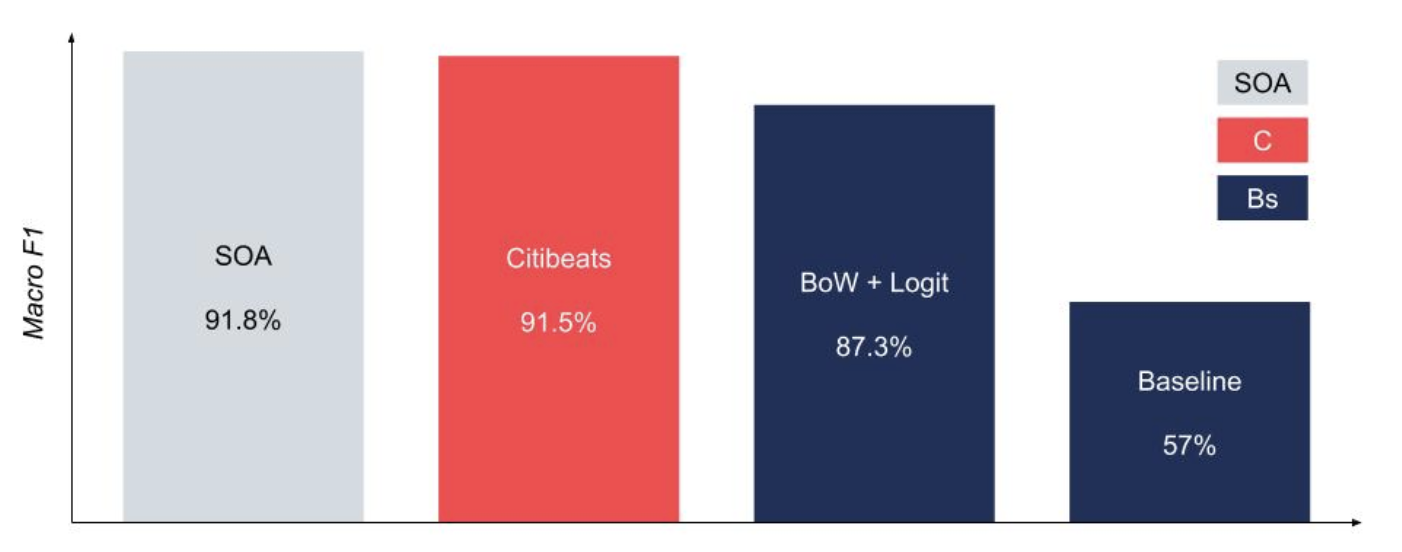
\includegraphics[scale=0.45]{figures/Figure 1.png}}

\end{frame}


\begin{frame}{Limitations of Rule-Based Systems in NLP}

\begin{stepitemize}
  \item \textbf{Static Rules}
    \begin{itemize}
      \item Require updates
      \item bootstrapping methods (Gupta et al., 2014) can help evolve rules.
    \end{itemize}

  \item \textbf{Multilingual Scalability}
    \begin{itemize}
      \item Challenging for multiple languages
      \item combining with translation tools and embedding alignment (Dou et al., 2016) can improve effectiveness.
    \end{itemize}

  \item \textbf{Too many rules}
    \begin{itemize}
      \item Specialized rules may quickly become outdated
      \item continuous updates and monitoring are expensive.
    \end{itemize}
\end{stepitemize}
\newline
\pause
\textbf{Once we have a strong baseline}: We may think about Machine Learning !

\end{frame}

\section{Bag Of Words}

\begin{frame}{Introduction to Bag of Words}

\begin{stepitemize}
\item \textbf{What is Bag of Words (BoW)?}
\begin{itemize}
  \item A simple and foundational text representation technique in NLP.
  \item Represents text data as a 'bag' (multiset) of words without considering grammar or word order but keeping multiplicity.
\end{itemize}

\item \textbf{How does it work?}
\begin{itemize}
  \item Texts are converted into a fixed-length vector of numbers.
  \item Each unique word in the text corpus corresponds to a feature (vector element).
  \item The frequency or presence of each word is then used to fill the vector.
\end{itemize}
\end{stepitemize}
\pause
\textbf{Note}: BoW is often the first step in feature extraction for NLP tasks.

\end{frame}

\begin{frame}{Term Frequency in Bag of Words}
\small
\begin{stepitemize}
\item \textbf{Term Frequency (TF)}
\begin{itemize}
  \item \textbf{Definition}: In the context of Bag of Words, Term Frequency measures how frequently a term occurs in a document.
  \item \textbf{Formal Representation}:
    \begin{itemize}
      \item Let \( d \) be a document in a corpus \( D \).
      \item Let \( w \) be a term (word) in document \( d \).
      \item The term frequency \( TF(w, d) \) is calculated as:
      \[ TF(w, d) = \text{Number of times word } w \text{ appears in document } d \]
    \end{itemize}
\end{itemize}

\item \textbf{Significance in Bag of Words}
\begin{itemize}
  \item TF is a fundamental concept in converting text to numerical format in BoW, representing the importance of each term in the document.
  \item It's a simple way to quantify and compare the occurrence of terms across different documents in a corpus.
\end{itemize}
\end{stepitemize}
\end{frame}

\begin{frame}[fragile]{Term Frequency Bag of Words with Scikit-Learn}
\small
\textbf{Generating a TF BoW Model}

Using Python's scikit-learn library to vectorize text data.

\textbf{Python Code}
\begin{tcolorbox}[colback=lightgray, colframe=lightgray,
                  boxsep=0mm, arc=1mm, boxrule=0mm,
                  left=1mm, right=1mm, top=1mm, bottom=1mm]
\begin{Verbatim}[fontsize=\scriptsize, bgcolor=lightgray]
from sklearn.feature_extraction.text import CountVectorizer

# Example sentences
sentences = ["The quick brown fox jumps over the lazy dog",
             "Never jump over the lazy dog quickly",
             "The fox is quick and brown"]

# Initialize CountVectorizer
vectorizer = CountVectorizer()

# Fit and transform the sentences
BoW_matrix = vectorizer.fit_transform(sentences)
print(BoW_matrix.toarray())
\end{Verbatim}
\end{tcolorbox}

\end{frame}


\begin{frame}[fragile]{Term Frequency Bag of Words with Scikit-Learn}
\small
\textbf{Python Code, results}
\begin{tcolorbox}[colback=lightgray, colframe=lightgray,
                  boxsep=0mm, arc=1mm, boxrule=0mm,
                  left=1mm, right=1mm, top=1mm, bottom=1mm]
\begin{Verbatim}[fontsize=\scriptsize, bgcolor=lightgray]
sentences = ["The quick brown fox jumps over the lazy dog",
             "Never jump over the lazy dog quickly",
             "The fox is quick and brown"]

Vocabulary: {'the': 12, 'quick': 10, 'brown': 1, 'fox': 3, 'jumps': 6,
              'over': 9,  'lazy': 7, 'dog': 2, 'never': 8,  'jump': 5,
              'quickly': 11, 'is': 4, 'and': 0}

tf_matrix:[[0 1 1 1 0 0 1 1 0 1 1 0 2]
           [0 0 1 0 0 1 0 1 1 1 0 1 1]
           [1 1 0 1 1 0 0 0 0 0 1 0 1]]
\end{Verbatim}
\end{tcolorbox}

\begin{itemize}
  \item The output matrix represents the term frequencies of each word in the sentences.
  \item Each column corresponds to a unique word in the combined sentences.
  \item Rows represent each sentence's word frequency vector.
\end{itemize}
\end{frame}


\begin{frame}{Limitations of Term Frequency BoW}

\begin{stepitemize}
  \item \textbf{Overemphasis on Frequent Words}:
    \begin{itemize}
      \item Common words like 'the' and 'is' may appear frequently but offer little value in understanding the unique context of each document.
      \item \textit{Example}: In our sentences, 'the' and 'quick' are frequent but not necessarily informative.
    \end{itemize}
\vspace{0.5em}
  \item \textbf{Ignoring Word Importance Across Documents}:
    \begin{itemize}
      \item TF BoW counts words in each document independently, not accounting for their importance or rarity across the entire document set.
      \item \textit{Example}: Words like 'fox' and 'dog', which might be key to understanding the specific content, are treated the same as common words.
    \end{itemize}
\end{stepitemize}
\end{frame}

\begin{frame}{Term Frequency-Inverse Document Frequency (TF-IDF)}
\begin{stepitemize}

\item \textbf{What is TF-IDF?}
\newline
It enhances the basic TF by considering not only the frequency of a word in a single document but also its frequency across multiple documents.

\item \textbf{Formal Definition}
\begin{itemize}
  \item Let \( w \) be a word, \( d \) a document, and \( D \) the corpus of documents.
  \item The TF-IDF value is calculated as:
  \[ \text{TF-IDF}(w, d, D) = TF(w, d) \times IDF(w, D) \]
  \item Where \( IDF(w, D) \) (Inverse Document Frequency) is defined as:
  \[ IDF(w, D) = \log \left(\frac{\text{Total number of documents in } D}{\text{Number of documents containing word } w}\right) \]
\end{itemize}
\end{stepitemize}
\end{frame}

\begin{frame}{Term Frequency-Inverse Document Frequency (TF-IDF)}

\textbf{Differences from TF BoW}
\begin{stepitemize}
  \item \textbf{Word Significance}: TF-IDF decreases the weight of words that occur frequently across many documents (common words), emphasizing words that are unique to specific documents.
  \item \textbf{Contextual Importance}: Unlike TF, which treats all terms equally, TF-IDF provides a way to assess the relevance of terms in the context of the entire corpus.
\end{stepitemize}
\pause
TF-IDF is widely used in information retrieval and text mining to reflect how important a word is to a document in a collection.

\end{frame}

\begin{frame}[fragile]{TF-IDF with Scikit-Learn}
\small
\textbf{Generating a TF-IDF Model}

Using Python's scikit-learn library to apply TF-IDF vectorization to data.

\textbf{Python Code}

\begin{tcolorbox}[colback=lightgray, colframe=lightgray,
                  boxsep=0mm, arc=1mm, boxrule=0mm,
                  left=1mm, right=1mm, top=1mm, bottom=1mm]
\begin{Verbatim}[fontsize=\scriptsize, bgcolor=lightgray]
from sklearn.feature_extraction.text import TfidfVectorizer

# Example sentences
sentences = ["The quick brown fox jumps over the lazy dog",
             "Never jump over the lazy dog quickly",
             "The fox is quick and brown"]

# Initialize TfidfVectorizer
vectorizer = TfidfVectorizer()

# Fit and transform the sentences
tfidf_matrix = vectorizer.fit_transform(sentences)

# Print the resulting matrix
print(tfidf_matrix.toarray())
\end{Verbatim}
\end{tcolorbox}

\end{frame}

\begin{frame}[fragile]{TF-IDF with Scikit-Learn}
\small
\textbf{Python Code, results}
\begin{tcolorbox}[colback=lightgray, colframe=lightgray,
                  boxsep=0mm, arc=1mm, boxrule=0mm,
                  left=1mm, right=1mm, top=1mm, bottom=1mm]
\begin{Verbatim}[fontsize=\scriptsize, bgcolor=lightgray]
sentences = ["The quick brown fox jumps over the lazy dog",
             "Never jump over the lazy dog quickly",
             "The fox is quick and brown"]

Vocabulary: {'the': 12, 'quick': 10, 'brown': 1, 'fox': 3, 'jumps': 6,
              'over': 9,  'lazy': 7, 'dog': 2, 'never': 8,  'jump': 5,
              'quickly': 11, 'is': 4, 'and': 0}

tf_matrix:[[0 1 1 1 0 0 1 1 0 1 1 0 2]
           [0 0 1 0 0 1 0 1 1 1 0 1 1]
           [1 1 0 1 1 0 0 0 0 0 1 0 1]]
tf_idf_matrix:
[[0.  0.3 0.3 0.3 0.  0.  0.4 0.3 0.  0.3 0.3 0.  0.5]
 [0.  0.  0.3 0.  0.  0.4 0.  0.3 0.4 0.3 0.  0.4 0.3]
 [0.5 0.4 0.  0.4 0.5 0.  0.  0.  0.  0.  0.4 0.  0.3]]
\end{Verbatim}
\end{tcolorbox}
\end{frame}

\begin{frame}{Limitations of TF-IDF and Motivation for BM25}
\small
\begin{stepitemize}
\item \textbf{Term Saturation}
\begin{itemize}
  \item Overemphasis on frequent terms due to linear term frequency assumption.
  \item \textit{E.g.}, "space" dominates over "exoplanets" in space-related texts.
\end{itemize}

\item \textbf{Document Length Bias}
\begin{itemize}
  \item Favors longer documents, overlooking shorter content's relevance.
  \item \textit{E.g.}, "Quantum computing" appears more relevant in longer papers.
\end{itemize}

\item \textbf{Query-Document Mismatch}
\begin{itemize}
  \item Lacks specific tuning for matching queries with document relevance.
  \item \textit{E.g.}, "Python" ambiguously interpreted in diverse contexts.
\end{itemize}
\end{stepitemize}
\pause
\textbf{Conclusion:} TF-IDF's simplistic approach leads to biased term weighting.

\end{frame}

\begin{frame}{BM25}
\begin{stepitemize}
\item \textbf{What is BM25?}\newline
It enhances TF-IDF balancing the term frequency with document length and query-document relevance.

\item \textbf{Formal Definition}
\begin{itemize}
  \item Given a sentence \( W \) containing terms \( w_1, w_2, ..., w_n \), the BM25 score of a document \( d \) is:
  \[ \text{Score}(d, W) = \sum_{i=1}^{n} IDF(w_i) \times \frac{tf(w_i, d) \times (k_1 + 1)}{tf(w_i, D) + k_1 \times (1 - b + b \times \frac{|d|}{\text{avgdl}})} \]
  \item Where \( tf(w_i, d) \) is \( w_i \)'s frequency in \( d \), \( |d| \) is the length of the document, and avgdl is the average document length in the corpus. \( k_1 \) and \( b \) are free parameters, usually chosen empirically.
  \item Where \( IDF(w_i) = ln(\frac{N - n(w_i) + 0.5}{n(w_i) + 0.5} + 1)\), \( N \) is the number of documents and \(n(w_i)\) the number of documents containing \(w_i\)
\end{itemize}
\end{stepitemize}
\end{frame}

\begin{frame}{Differences with TF-IDF}

\textbf{Key Differences Between BM25 and TF-IDF}

\begin{itemize}
  \item \textbf{TF / (TF + k), the backbone of BM25}
    \begin{itemize}
      \item \textit{Term saturation}: now limited by 1. the higher k the lower it reaches 1.
      \item \textit{Document length}: let k depends on length of the document as k =\( |d| \)/avgdl, the longer the document, the more it will penalize the score. The value of b wgives the speed of the growth.
    \end{itemize}

  \item \textbf{Document Length Normalization}
    \begin{itemize}
      \item \textit{BM25}: k depends on length of the document as k =\( |d| \)/avgdl
    \end{itemize}

\end{itemize}

\textbf{Conclusion:} BM25 addresses several key limitations of TF-IDF, making it more suitable for modern information retrieval systems.

\end{frame}

\begin{frame}{Illustrations of TF / (TF + k)}

\textbf{BM25 Formula}
\[ \text{Score}(d, W) = \sum_{i=1}^{n} IDF(w_i) \times \frac{f(w_i, d) \times (k_1 + 1)}{f(w_i, D) + k_1 \times (1 - b + b \times \frac{|d|}{\text{avgdl}})} \]

\textbf{TF-IDF Formula}
\[ \text{TF-IDF}(w, d, D) = TF(w, d) \times IDF(w, D) \]

\begin{figure}
  \centering
  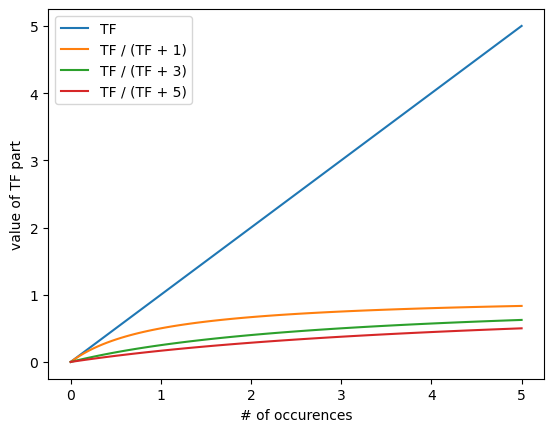
\includegraphics[width=0.5\textwidth]{figures/tf.png}
  \caption{Visual Representation of TF Concept}
\end{figure}

\end{frame}

\begin{frame}{Illustrations of IDFs}

\textbf{BM25 Formula}
\[ IDF(w_i) = ln(\frac{N - n(w_i) + 0.5}{n(w_i) + 0.5} + 1) \]

\textbf{TF-IDF Formula}
\[ IDF(w, D) = \log \left(\frac{\text{Total number of documents in } D}{\text{Number of documents containing word } w}\right) \]

\begin{figure}
  \centering
  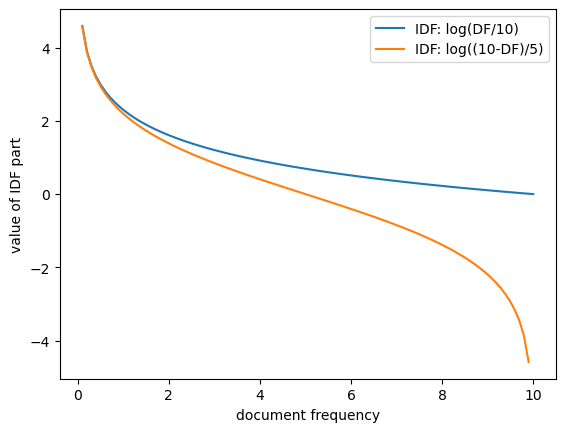
\includegraphics[width=0.5\textwidth]{figures/idf.png}
  \caption{Visual Representation of IDF Concept}
\end{figure}

\end{frame}


\begin{frame}[fragile]{BM25 with Scikit-Learn}
\small
\textbf{Generating a BM25 representation}

Using Python's scikit-learn library and some functions to compute BM25.

\textbf{Python Code}

\begin{tcolorbox}[colback=lightgray, colframe=lightgray,
                  boxsep=0mm, arc=1mm, boxrule=0mm,
                  left=1mm, right=1mm, top=1mm, bottom=1mm]
\begin{Verbatim}[fontsize=\scriptsize, bgcolor=lightgray]
from sklearn.feature_extraction.text import CountVectorizer

# Example sentences
sentences = ["The quick brown fox jumps over the lazy dog",
             "Never jump over the lazy dog quickly",
             "The fox is quick and brown"]

# Initialize CountVectorizer
vectorizer = CountVectorizer()

# Fit and transform the sentences
tf_matrix = vectorizer.fit_transform(sentences)
\end{Verbatim}
\end{tcolorbox}

\end{frame}

\begin{frame}[fragile]{BM25 with Scikit-Learn}
\small
\begin{tcolorbox}[colback=lightgray, colframe=lightgray,
                  boxsep=0mm, arc=1mm, boxrule=0mm,
                  left=1mm, right=1mm, top=1mm, bottom=1mm]
\begin{Verbatim}[fontsize=\scriptsize, bgcolor=lightgray]
from math import log
import numpy as np

def compute_idf(corpus):
    N = len(corpus)
    idf_dict = {}
    for document in corpus:
        for term in set(document.split()):
            idf_dict[term] = idf_dict.get(term, 0) + 1
    for term, count in idf_dict.items():
        idf_dict[term] = log(N / float(count))
    return idf_dict

def bm25(tf, idf, avgdl, dl, b=0.75, k1=1.5):
    return idf * (tf * (k1 + 1))/(tf + k1 * (1 - b + b * (dl / avgdl)))
\end{Verbatim}
\end{tcolorbox}

\end{frame}

\begin{frame}[fragile]{BM25 with Scikit-Learn}
\small
\begin{tcolorbox}[colback=lightgray, colframe=lightgray,
                  boxsep=0mm, arc=1mm, boxrule=0mm,
                  left=1mm, right=1mm, top=1mm, bottom=1mm]
\begin{Verbatim}[fontsize=\scriptsize, bgcolor=lightgray]

# Calculate IDF
idf_dict = compute_idf(sentences)
avgdl = np.mean([len(doc.split()) for doc in sentences])

# Calculate BM25
bm25_matrix = np.zeros((len(sentences), len(terms)))
for i, sentence in enumerate(sentences):
    dl = len(sentence.split())
    for j, term in enumerate(terms):
        tf = X[i, j]
        idf = idf_dict.get(term, 0)
        bm25_matrix[i, j] = bm25(tf, idf, avgdl, dl)

\end{Verbatim}
\end{tcolorbox}

\end{frame}

\begin{frame}[fragile]{BM25 with Scikit-Learn}
\small
\textbf{Python Code, results}
\begin{tcolorbox}[colback=lightgray, colframe=lightgray,
                  boxsep=0mm, arc=1mm, boxrule=0mm,
                  left=1mm, right=1mm, top=1mm, bottom=1mm]
\begin{Verbatim}[fontsize=\scriptsize, bgcolor=lightgray]
sentences = ["The quick brown fox jumps over the lazy dog",
             "Never jump over the lazy dog quickly",
             "The fox is quick and brown"]

Vocabulary: {'the': 12, 'quick': 10, 'brown': 1, 'fox': 3, 'jumps': 6,
              'over': 9,  'lazy': 7, 'dog': 2, 'never': 8,  'jump': 5,
              'quickly': 11, 'is': 4, 'and': 0}

tf_idf_matrix:
[[0.  0.3 0.3 0.3 0.  0.  0.4 0.3 0.  0.3 0.3 0.  0.5]
 [0.  0.  0.3 0.  0.  0.4 0.  0.3 0.4 0.3 0.  0.4 0.3]
 [0.5 0.4 0.  0.4 0.5 0.  0.  0.  0.  0.  0.4 0.  0.3]]

bm25_matrix:
[[0.  0.4 0.4 0.4 0.  0.  1.  0.4 0.  0.4 0.4 0.  0.5]
 [0.  0.  0.4 0.  0.  1.1 0.  0.4 0.  0.4 0.  1.1 0.4]
 [1.2 0.4 0.  0.4 1.2 0.  0.  0.  0.  0.  0.4 0.  0.4]]
\end{Verbatim}
\end{tcolorbox}
\end{frame}

\begin{frame}{Limitations of TF-IDF}

\textbf{TF-IDF Limitations}
\begin{itemize}
  \item \textbf{Term Frequency Bias}: Overemphasizes words that appear frequently, potentially overshadowing rare yet significant terms.
  \item \textbf{Document Length}: Fails to normalize for document length, potentially biasing towards longer documents.
  \item \textbf{Lack of Context and Semantics}: Treats each word independently without considering context or word meanings.
\end{itemize}
\end{frame}

\begin{frame}{Limitations of BM25}

\textbf{BM25 Limitations}
\begin{itemize}
  \item \textbf{Parameter Sensitivity}: The effectiveness of BM25 depends on the tuning of its parameters \( k_1 \) and \( b \), which may not be straightforward.
  \item \textbf{Still Context-Agnostic}: Like TF-IDF, BM25 does not account for word order, semantics, or the overall context of the query or document.
  \item \textbf{Complexity in Large Scale Applications}: Computationally more complex than TF-IDF, especially for very large document collections.
\end{itemize}

\textbf{Note}: Both methods, while foundational in information retrieval, have been partly superseded by more advanced NLP techniques that better understand context and semantics, like word embeddings and neural network models.

\end{frame}


\begin{frame}{QA}

\textbf{Open Discussion}
\begin{itemize}
  \item Feel free to ask questions or share your thoughts about today's topics.
  \item Any insights, experiences, or perspectives you'd like to discuss are welcome.
\end{itemize}

\end{frame}


\begin{frame}{Summary of Key Takeaways}

\begin{itemize}
  \item \textbf{Metrics and Evaluation}: Discussed various metrics and evaluation strategies to judge model quality.
  \item \textbf{Baselines in NLP}: Emphasized the importance of establishing baselines for comparison and model assessment.
  \item \textbf{Term Frequency's Role}: Understood its significance in text representation and limitations in context and semantics.
  \item \textbf{TF-IDF and BM25}: Explored their concepts, applications, and limitations.
  \item \textbf{BM25's Advantages}: Improved handling of term frequency and document length, but with its own set of challenges.
  \item \textbf{Evolving Landscape of NLP}: Recognized advancements beyond TF-IDF and BM25 towards more context-aware and semantic approaches in NLP.
\end{itemize}

\end{frame}




\end{document}
